% =========================================================================
% Chapter 4: Materials and Methods
% =========================================================================

\chapter{Materials and Methods}
\label{ch:methods}

Work was carried out at the Advanced Research Laboratory, Department of Zoology, University of Kashmir, Srinagar.

\section{Source of plant material}
\label{sec:plant_collection}

Whole plants of \textit{Dipsacus inermis} Wall.\ ex DC.\ were obtained from the Department of Botany, University of Kashmir (34.1280$^{\circ}$\,N, 74.8365$^{\circ}$\,E; \autoref{fig:collection_site}). Material was identified on morphological characters of the teasel capitulum and opposite stem leaves. Plants were washed in distilled water to remove soil, shade-dried at room temperature, chopped, and pulverised in a porcelain mortar and pestle to a coarse powder (\autoref{fig:dried_herb_tray}--\autoref{fig:lab_weighing}). The powder was stored in an airtight container, protected from light and moisture, until extraction.

\begin{figure}[hbt!]
  \centering
  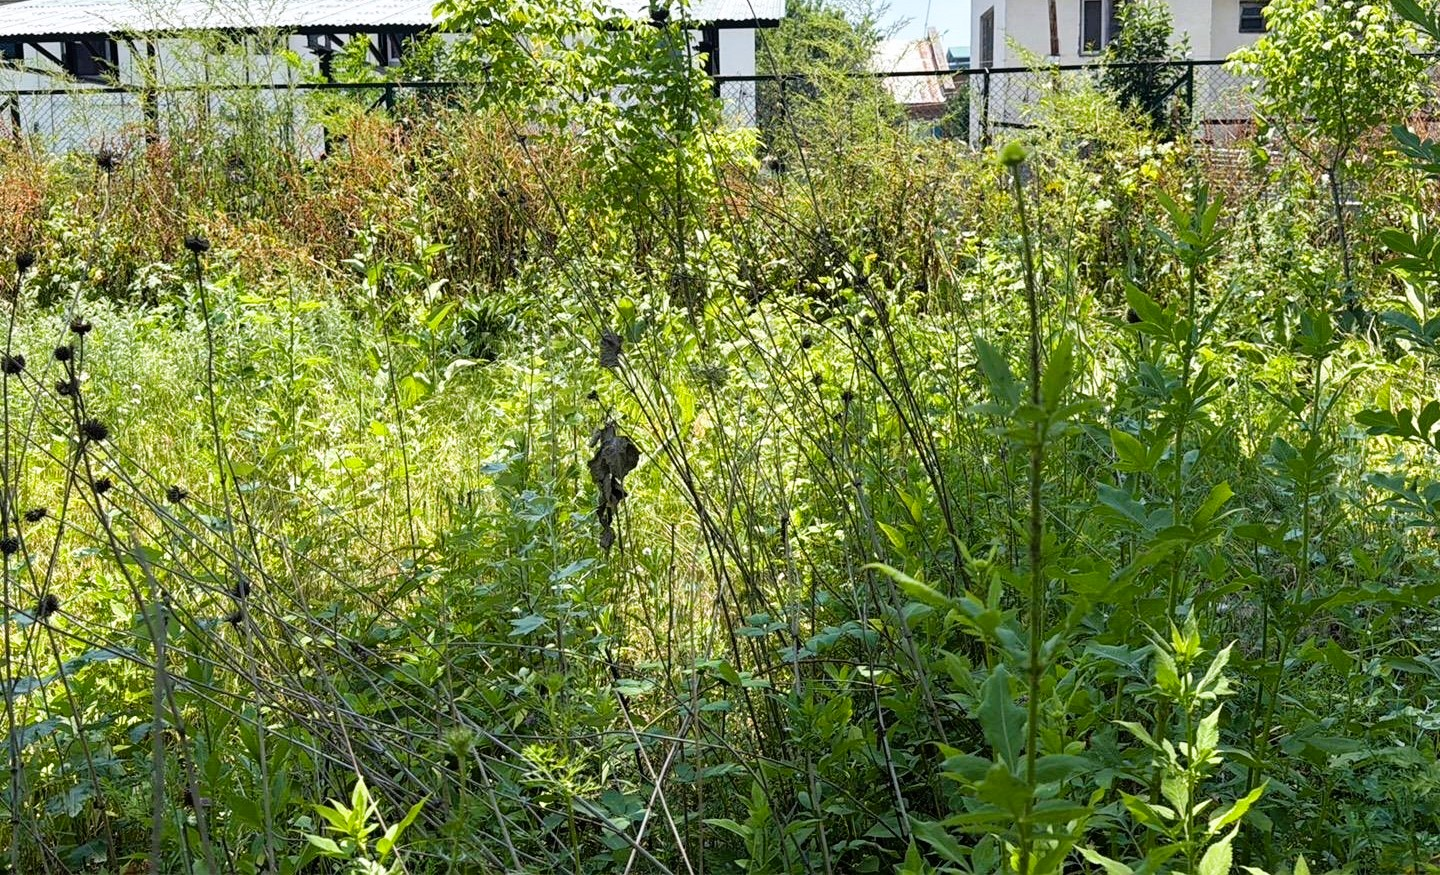
\includegraphics[width=0.72\textwidth]{figures/fig_collection_site.jpg}
  \caption{\textit{Dipsacus inermis} collected through the Department of Botany, University of Kashmir (34.1280$^{\circ}$\,N, 74.8365$^{\circ}$\,E).}
  \label{fig:collection_site}
\end{figure}

\begin{figure}[hbt!]
  \centering
  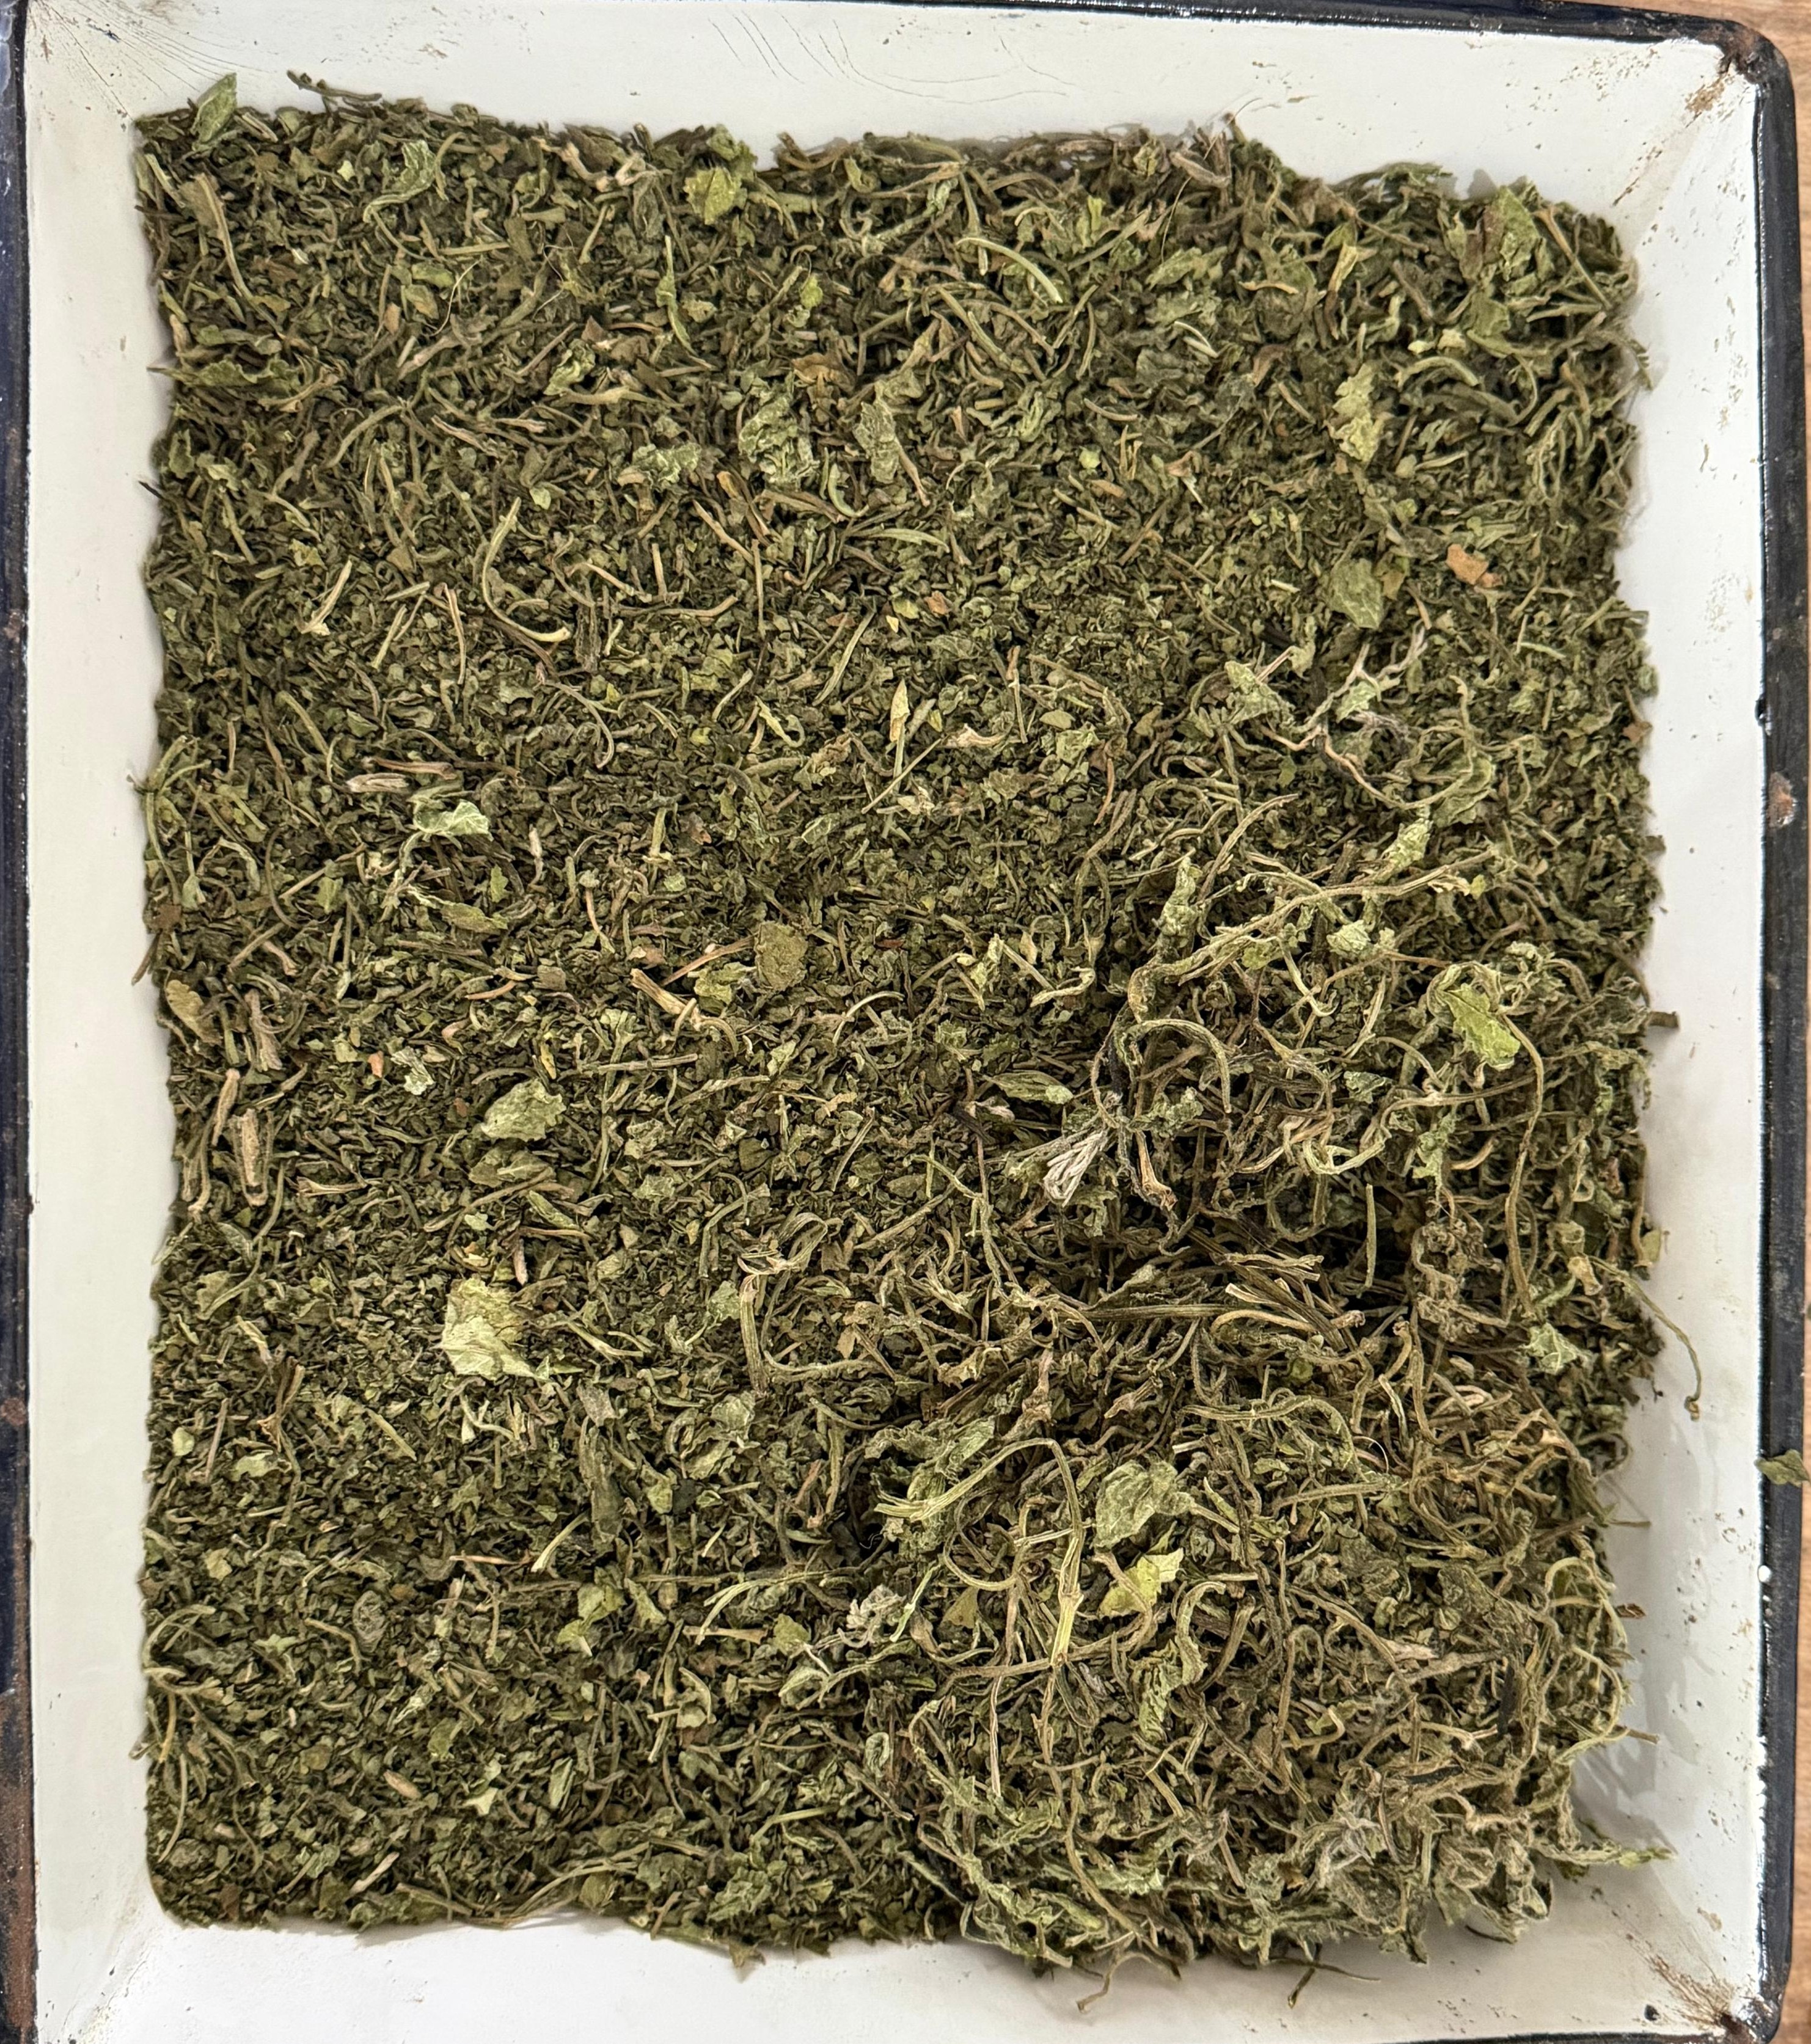
\includegraphics[width=0.62\textwidth]{figures/fig_dried_herb_tray.jpg}
  \caption{Shade-dried, chopped whole-plant \textit{D.\ inermis} in a metal tray before grinding.}
  \label{fig:dried_herb_tray}
\end{figure}

\begin{figure}[hbt!]
  \centering
  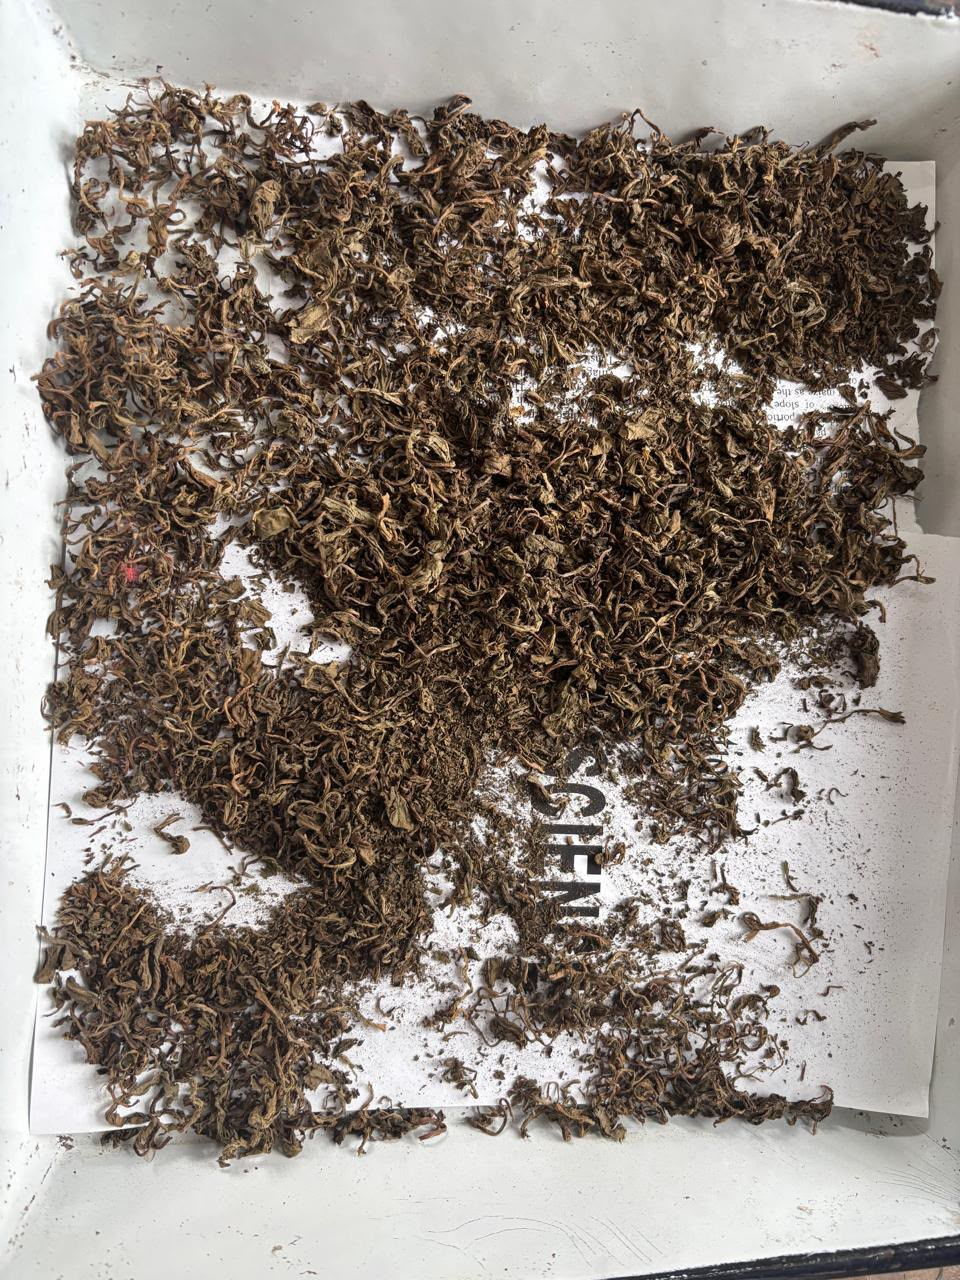
\includegraphics[width=0.62\textwidth]{figures/fig1_plant_material.jpg}
  \caption{Shade-dried whole-plant material of \textit{Dipsacus inermis} before grinding.}
  \label{fig:plant_material}
\end{figure}

\begin{figure}[hbt!]
  \centering
  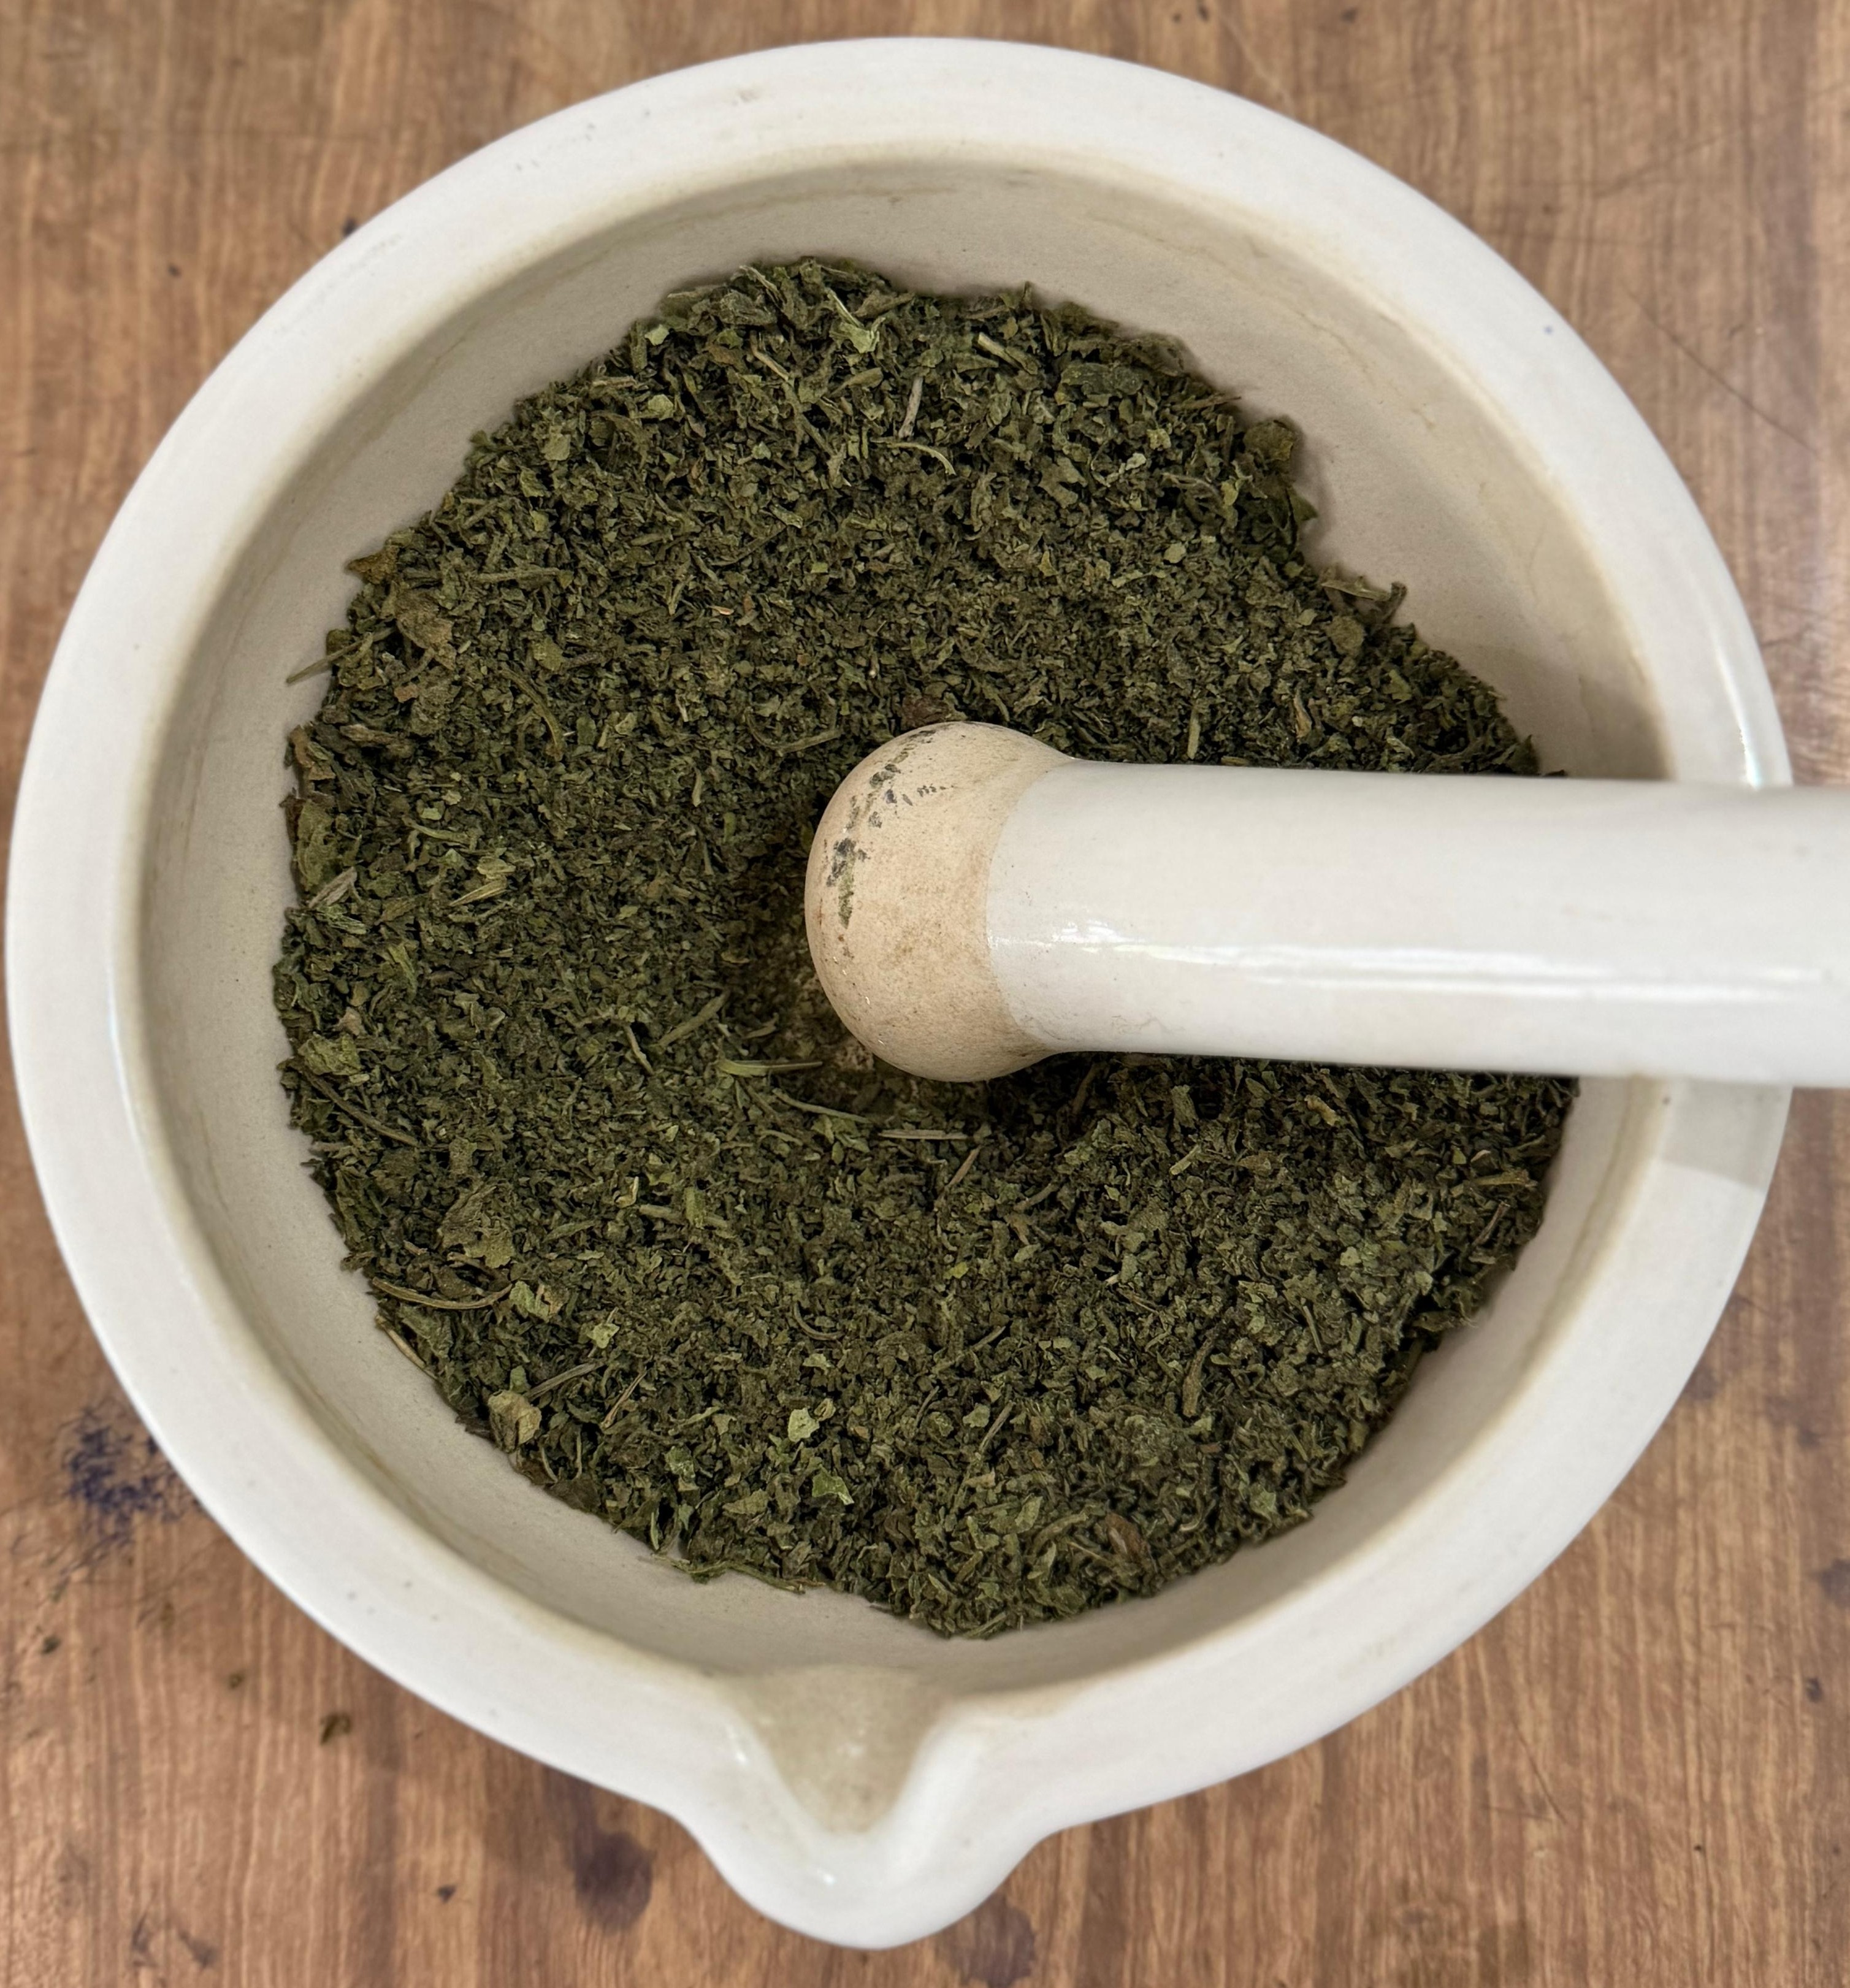
\includegraphics[width=0.55\textwidth]{figures/fig_chopped_mortar.jpg}
  \caption{Chopped dried \textit{D.\ inermis} in a porcelain mortar before fine grinding.}
  \label{fig:chopped_mortar}
\end{figure}

\begin{figure}[hbt!]
  \centering
  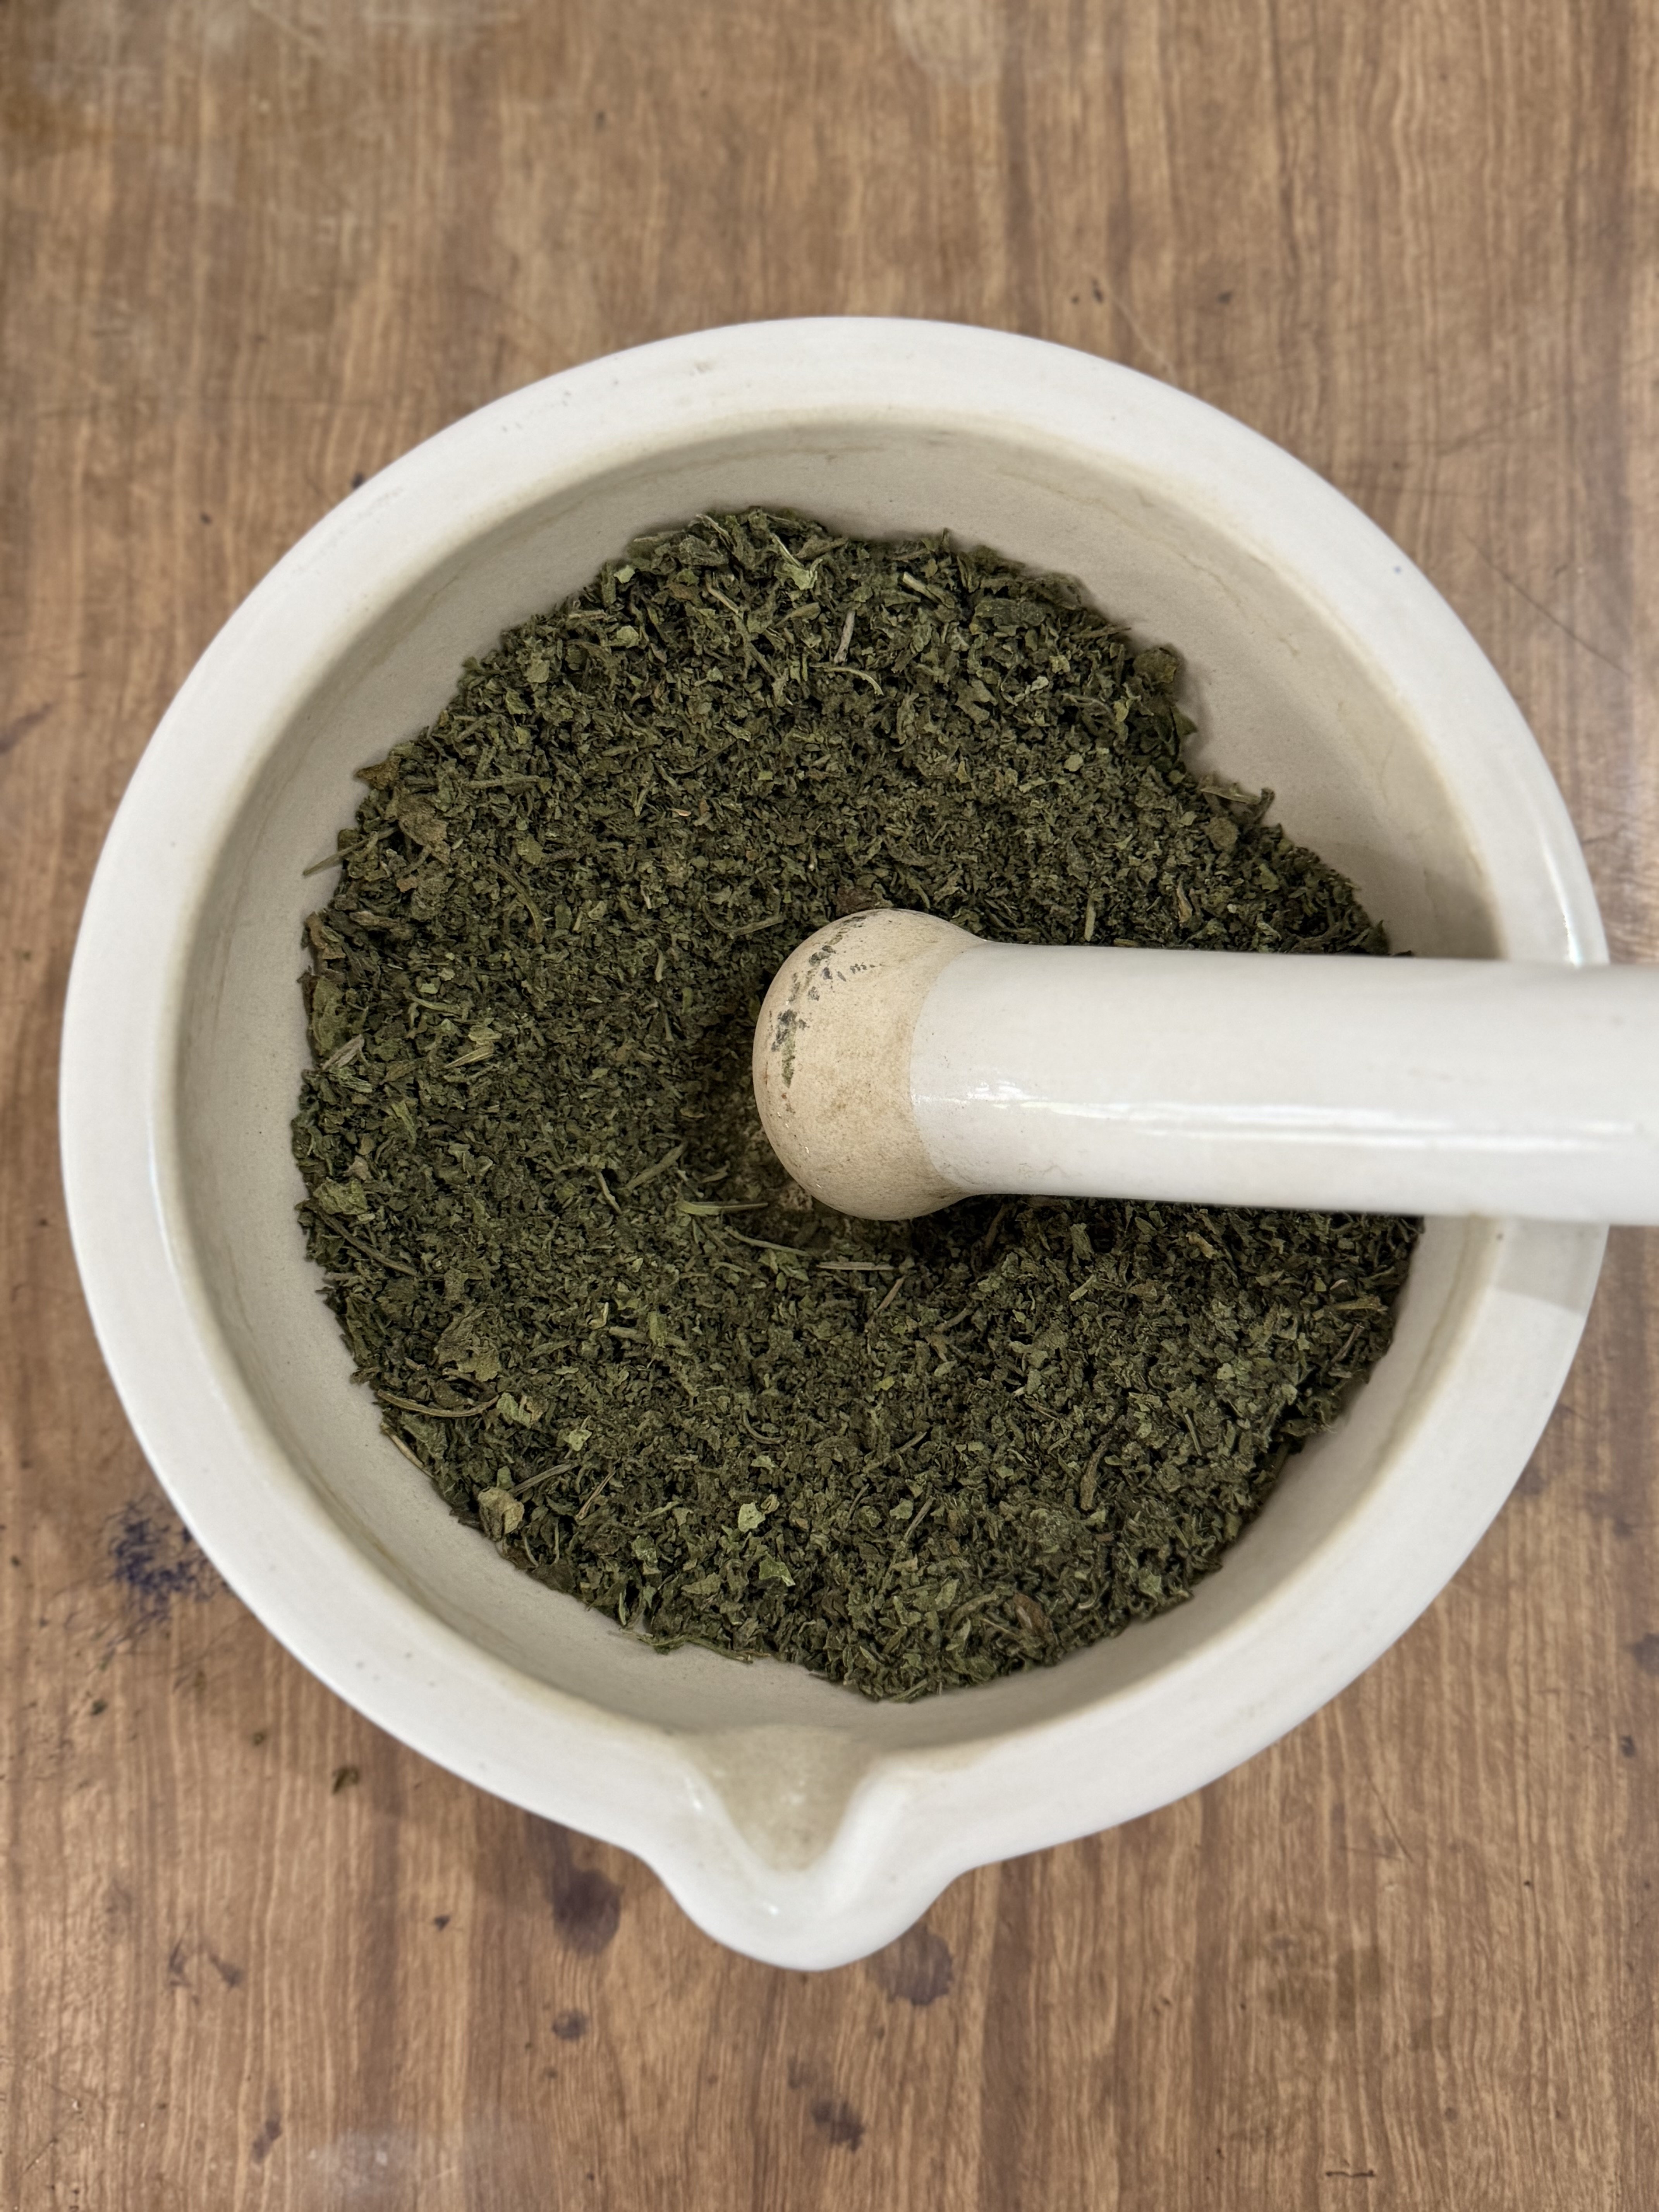
\includegraphics[width=0.62\textwidth]{figures/fig2_mortar_pestle.jpg}
  \caption{Powdering of dried \textit{D.\ inermis} in a porcelain mortar and pestle.}
  \label{fig:mortar_pestle}
\end{figure}

\begin{figure}[hbt!]
  \centering
  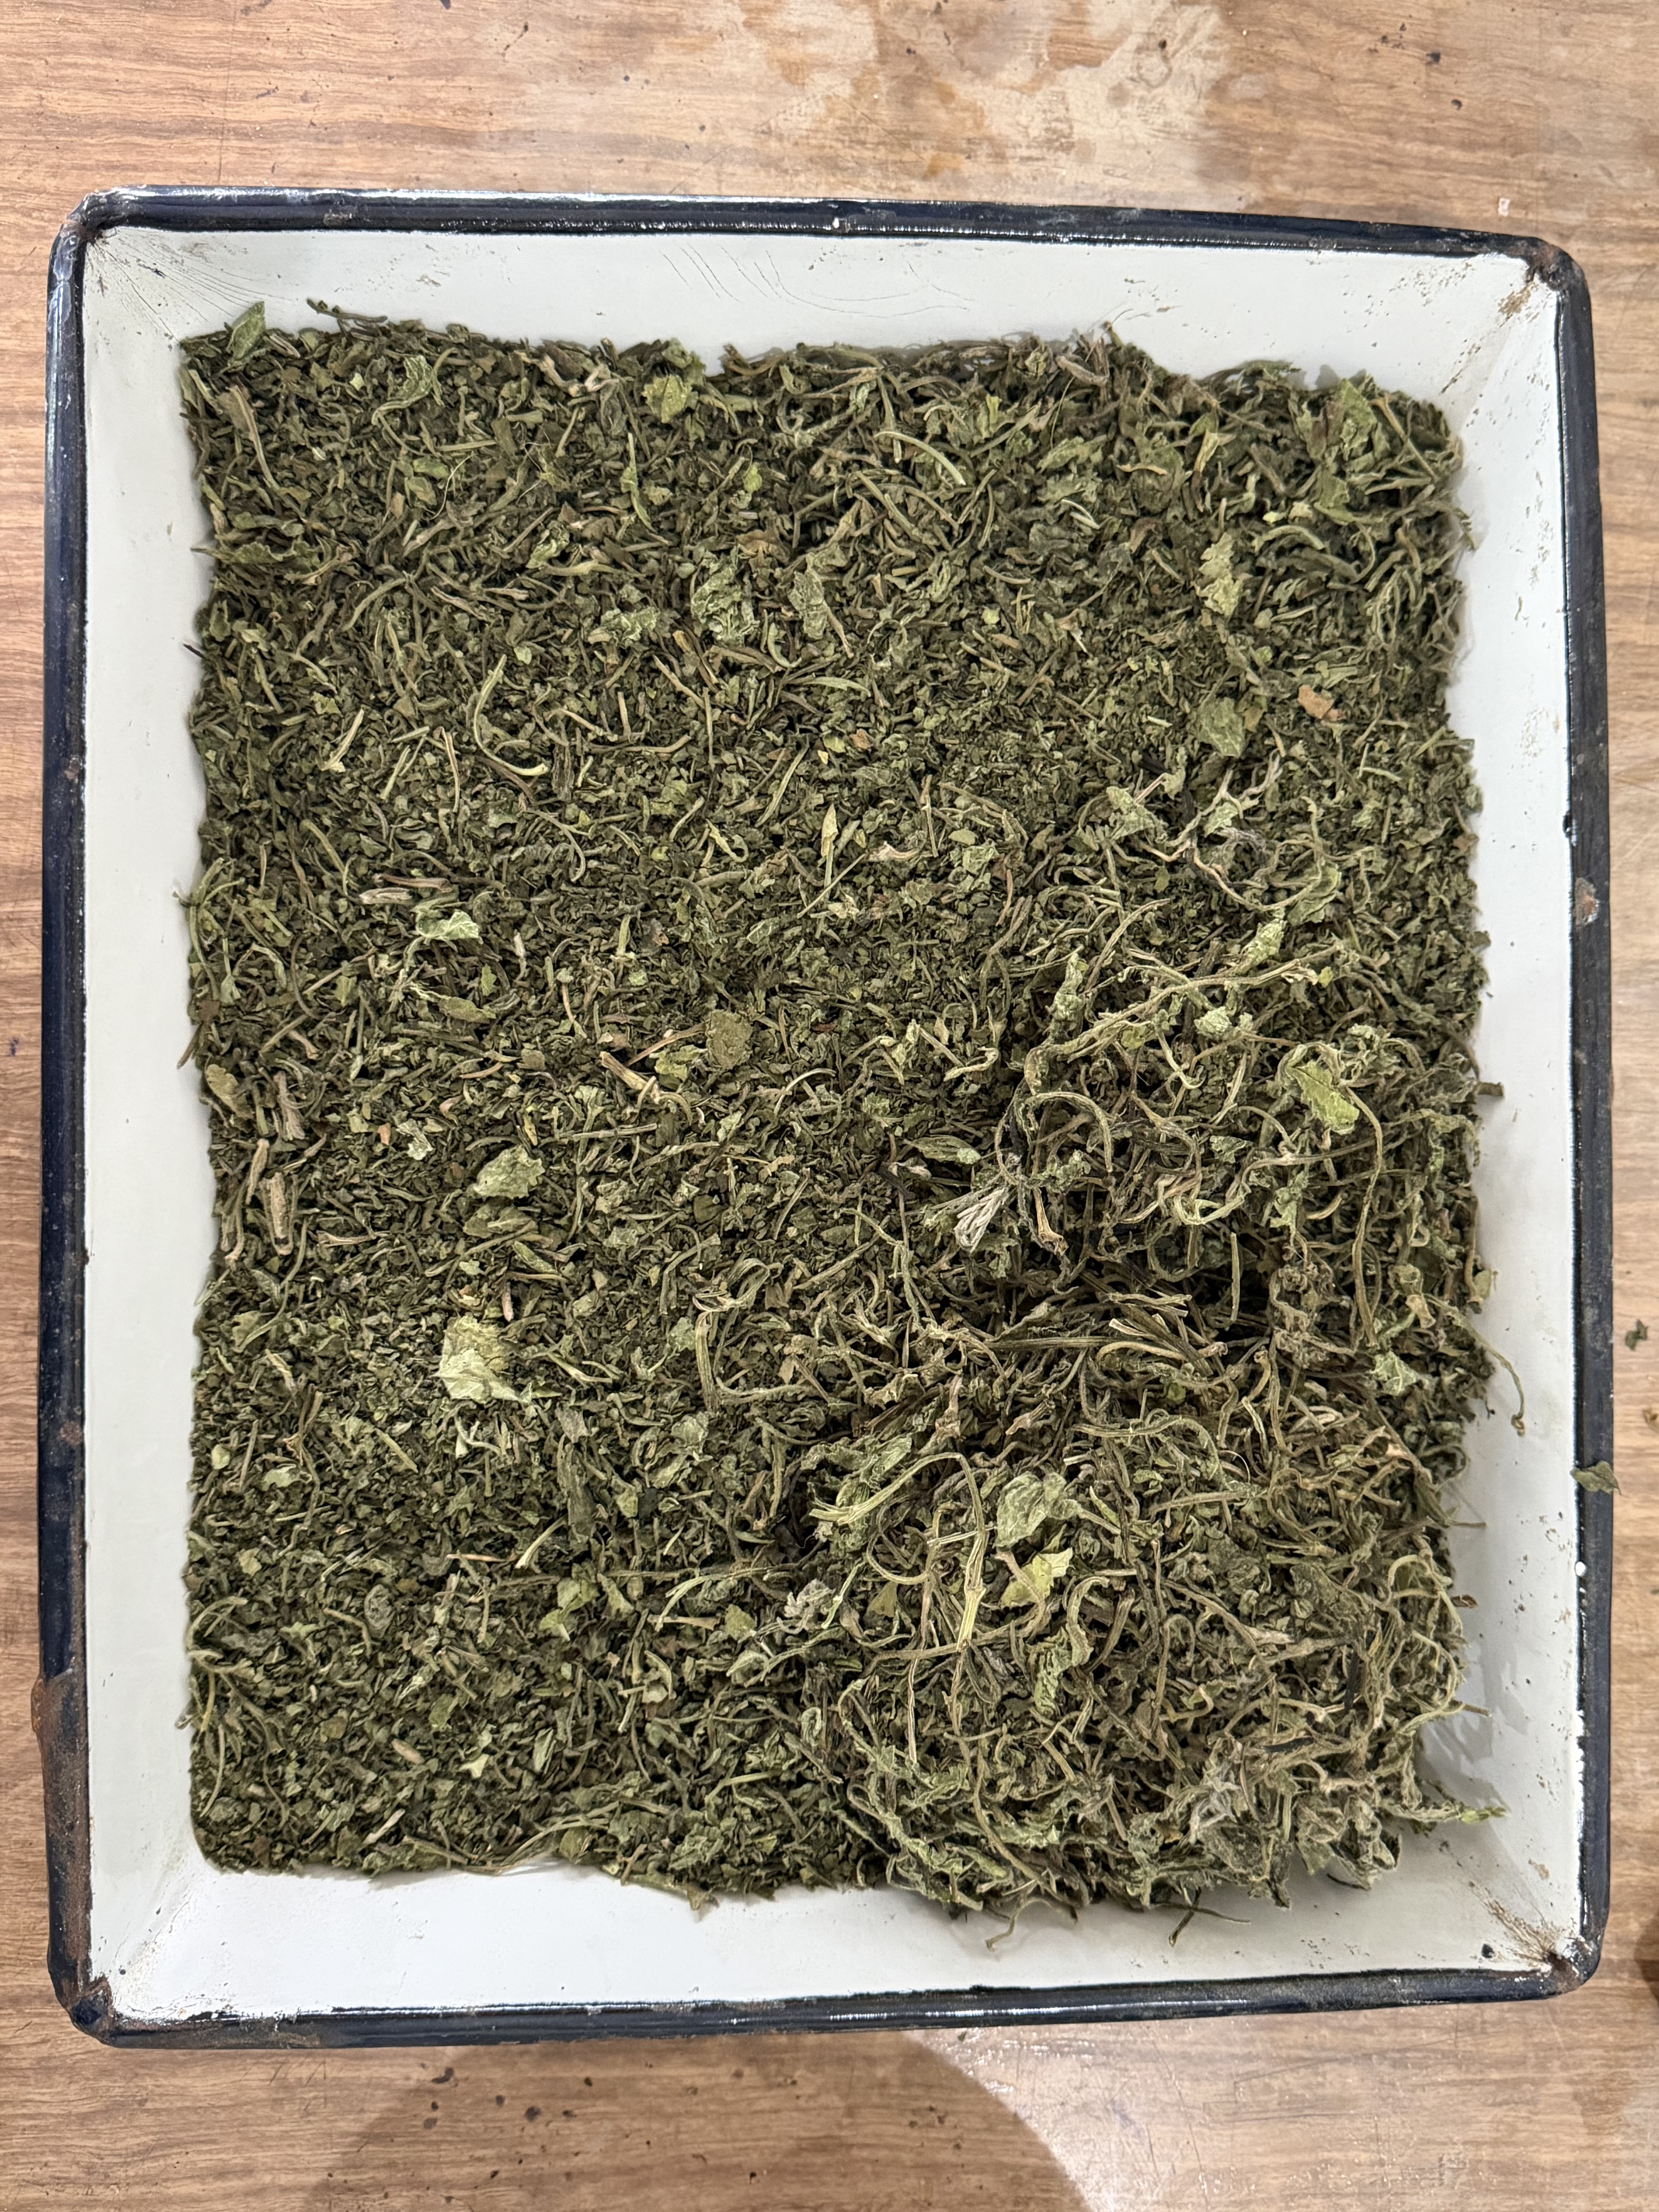
\includegraphics[width=0.62\textwidth]{figures/fig3_powdered_plant.jpg}
  \caption{Coarse powder of \textit{D.\ inermis} prepared for aqueous extraction.}
  \label{fig:powdered_plant}
\end{figure}

\begin{figure}[hbt!]
  \centering
  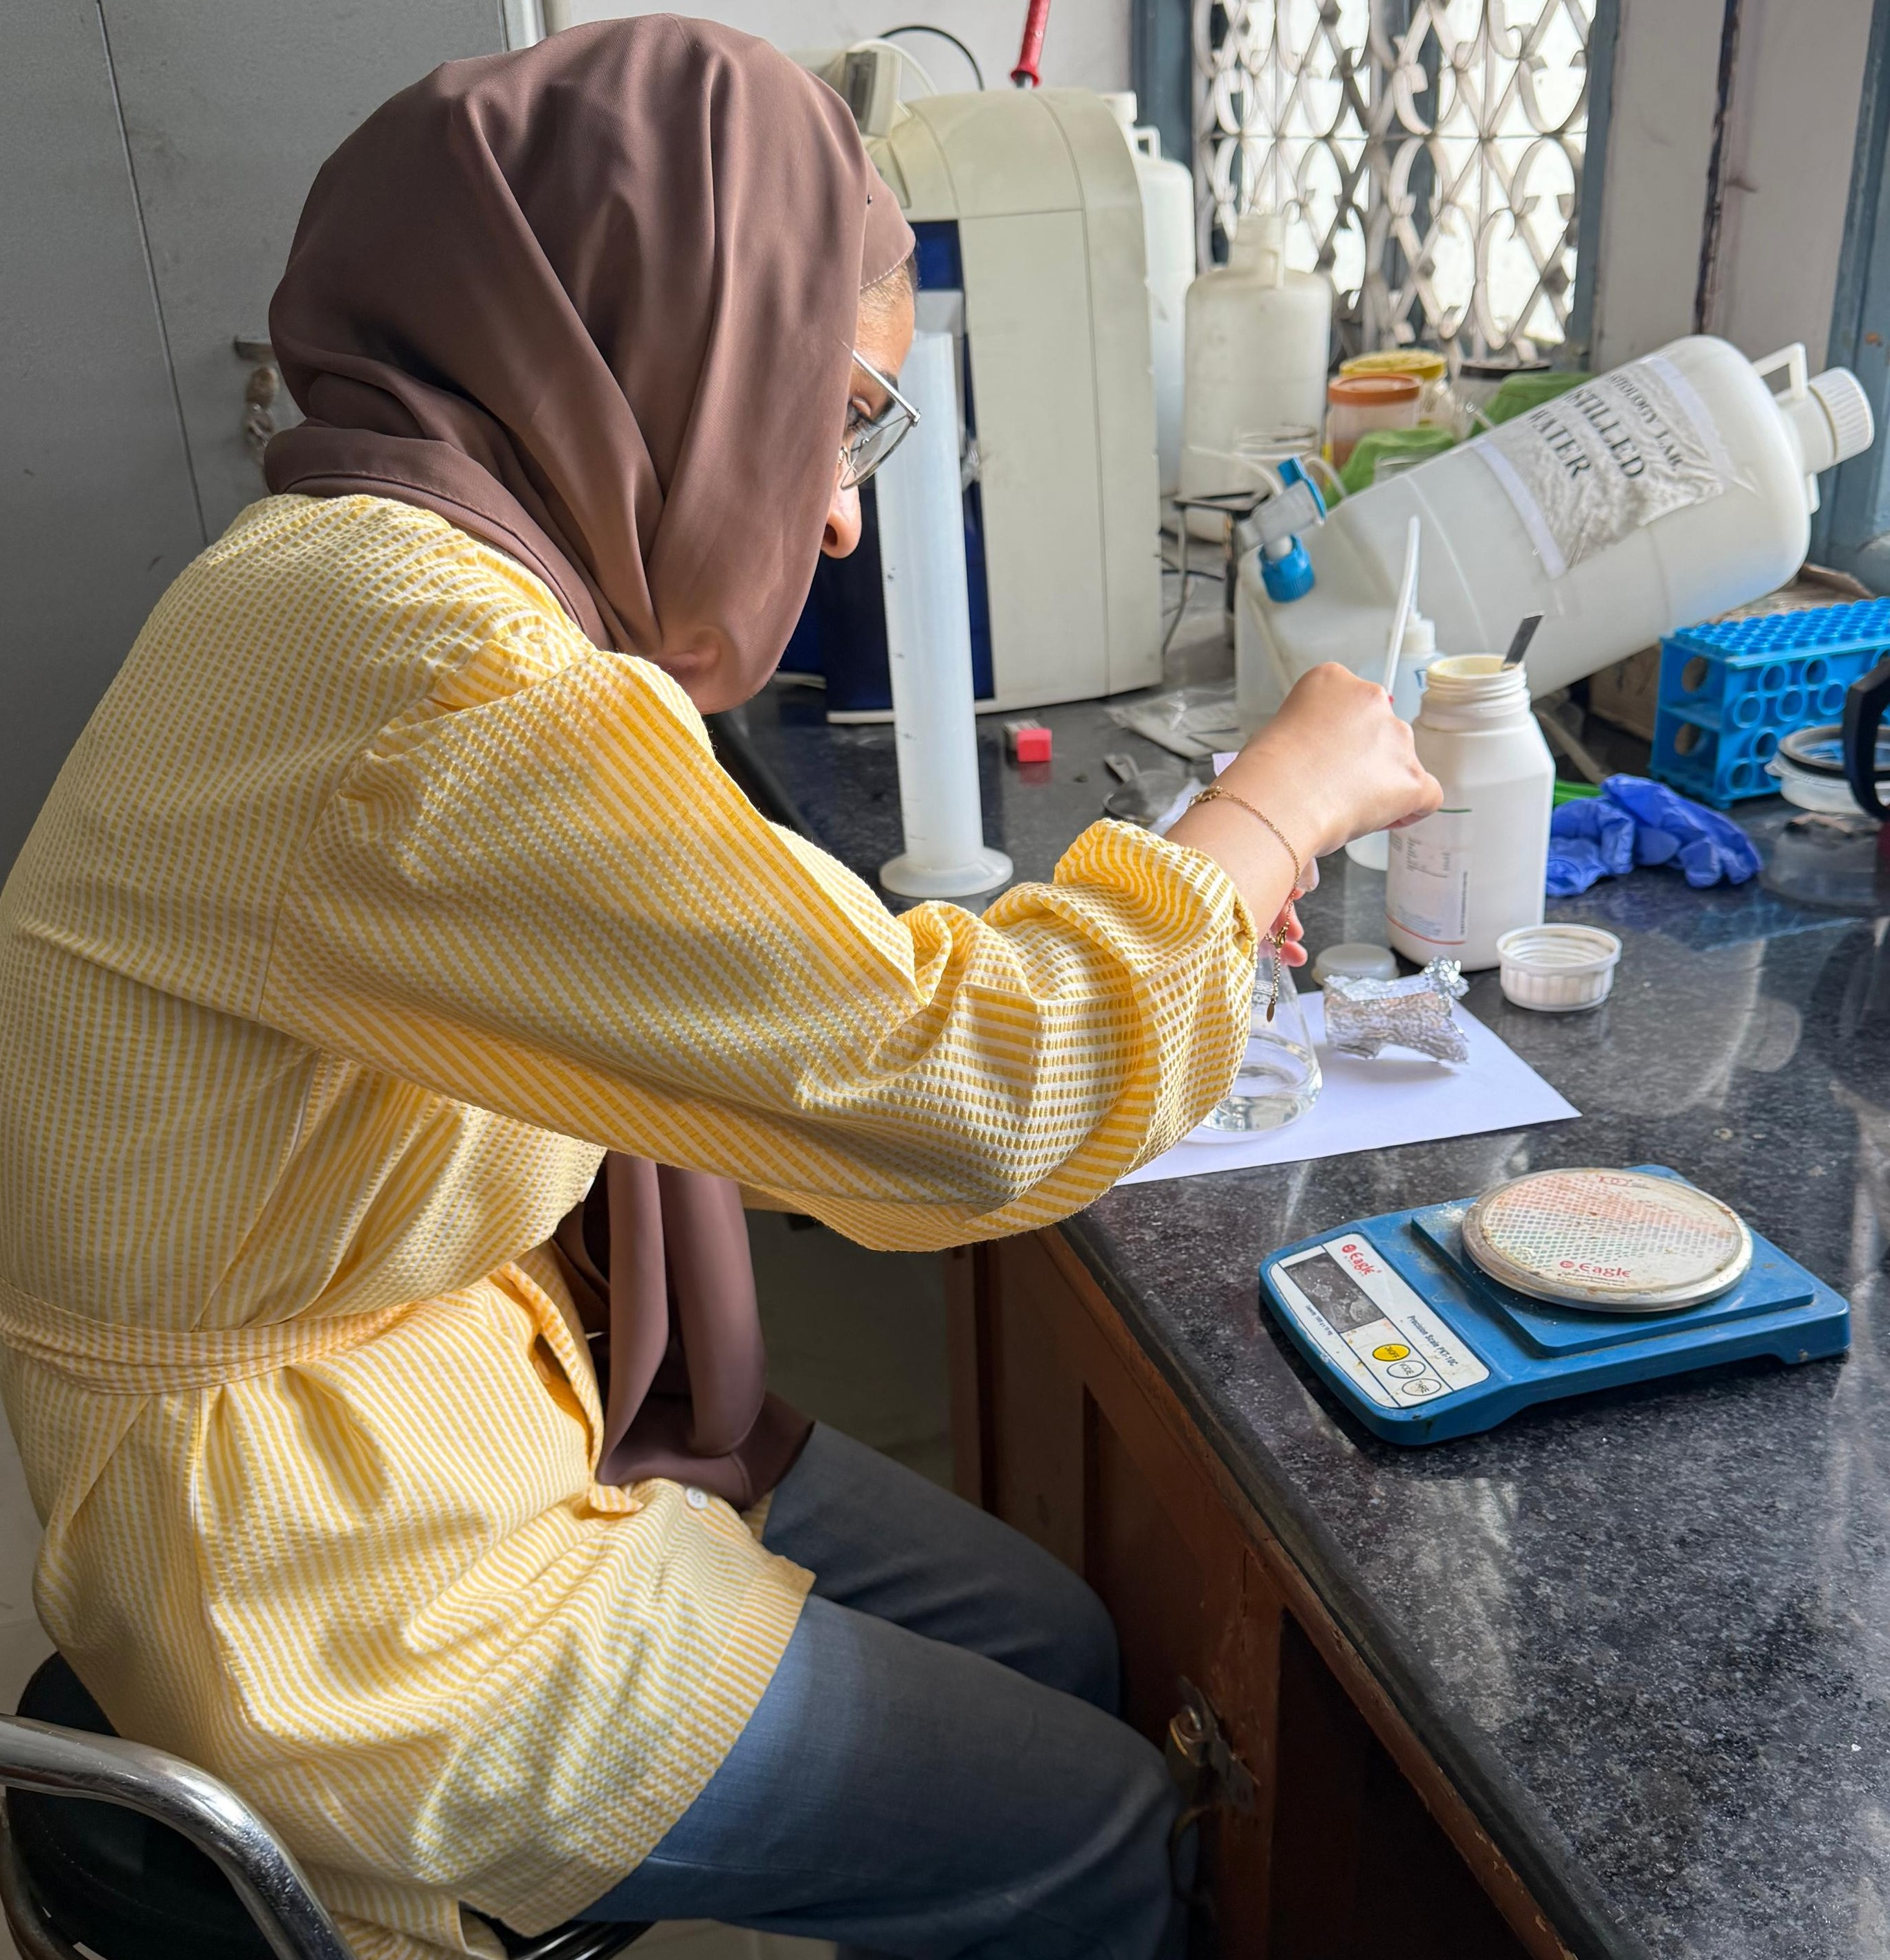
\includegraphics[width=0.62\textwidth]{figures/fig_lab_weighing.jpg}
  \caption{Weighing of dried plant material at the Advanced Research Laboratory, Department of Zoology.}
  \label{fig:lab_weighing}
\end{figure}

\section{Preparation of aqueous extract}
\label{sec:aqueous_extraction}

Powdered plant material was extracted in distilled water (\autoref{fig:extraction_setup}--\autoref{fig:soxhlet_bench}). The liquor was filtered through muslin cloth and then through Whatman No.\ 1 filter paper. The filtrate was used as the aqueous extract for phytochemical tests and for the disc-diffusion assay.

\begin{figure}[hbt!]
  \centering
  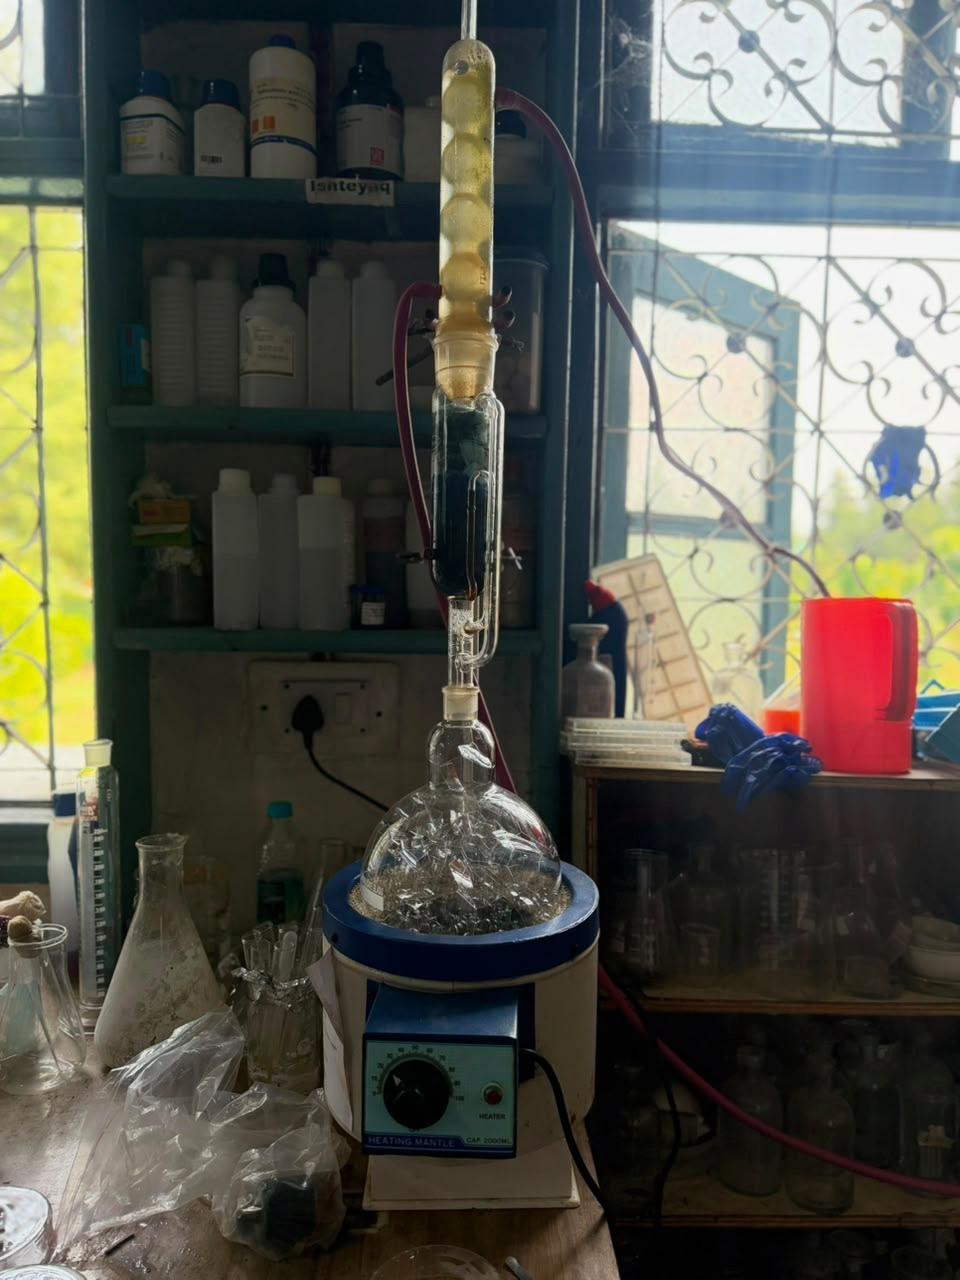
\includegraphics[width=0.62\textwidth]{figures/fig4_extraction_setup.jpg}
  \caption{Aqueous extraction of powdered \textit{D.\ inermis} in distilled water.}
  \label{fig:extraction_setup}
\end{figure}

\begin{figure}[hbt!]
  \centering
  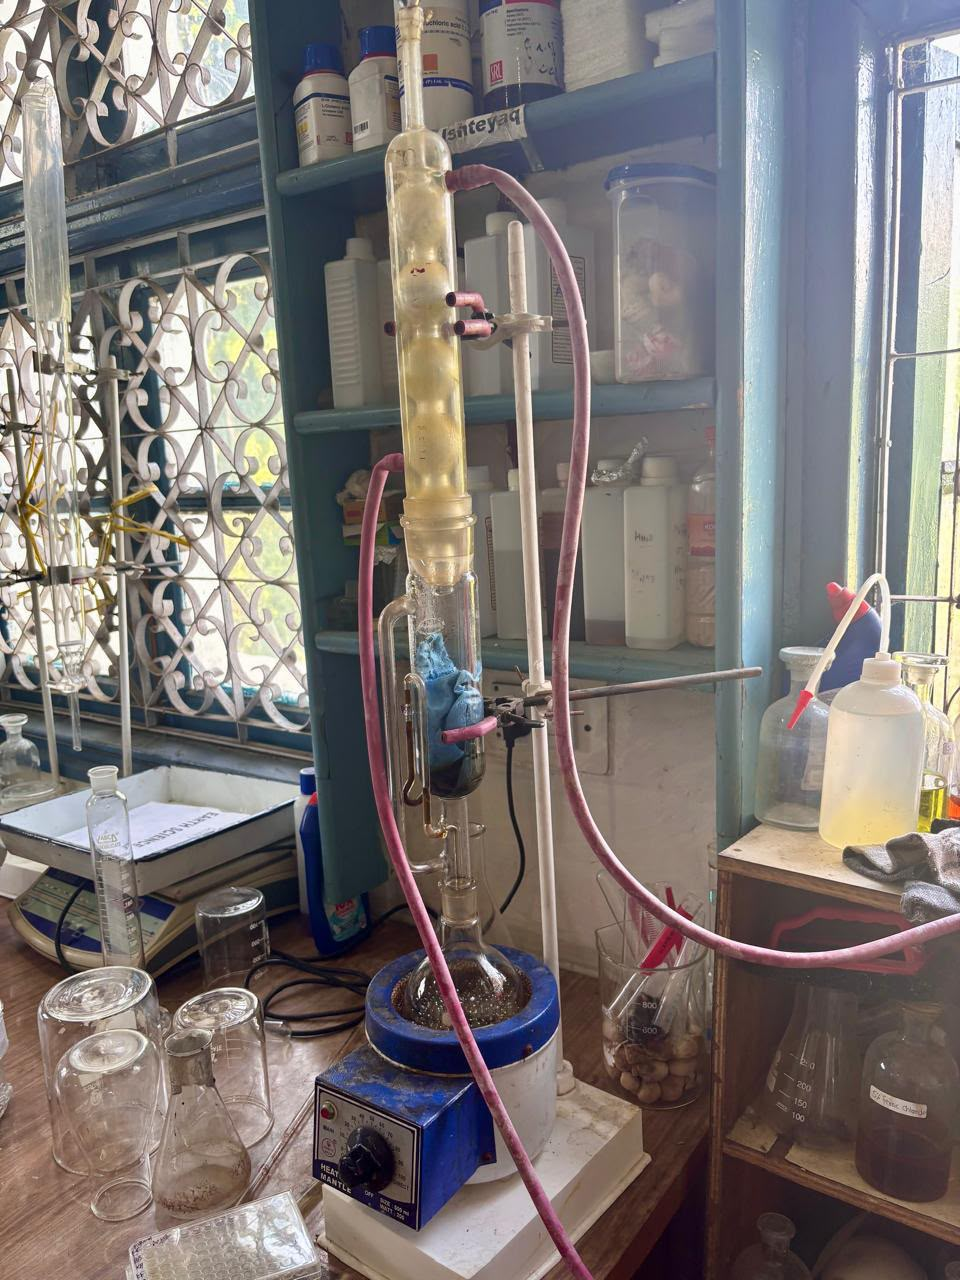
\includegraphics[width=0.62\textwidth]{figures/fig5_reflux_assembly.jpg}
  \caption{Laboratory extraction assembly during preparation of the aqueous extract.}
  \label{fig:reflux_assembly}
\end{figure}

\begin{figure}[hbt!]
  \centering
  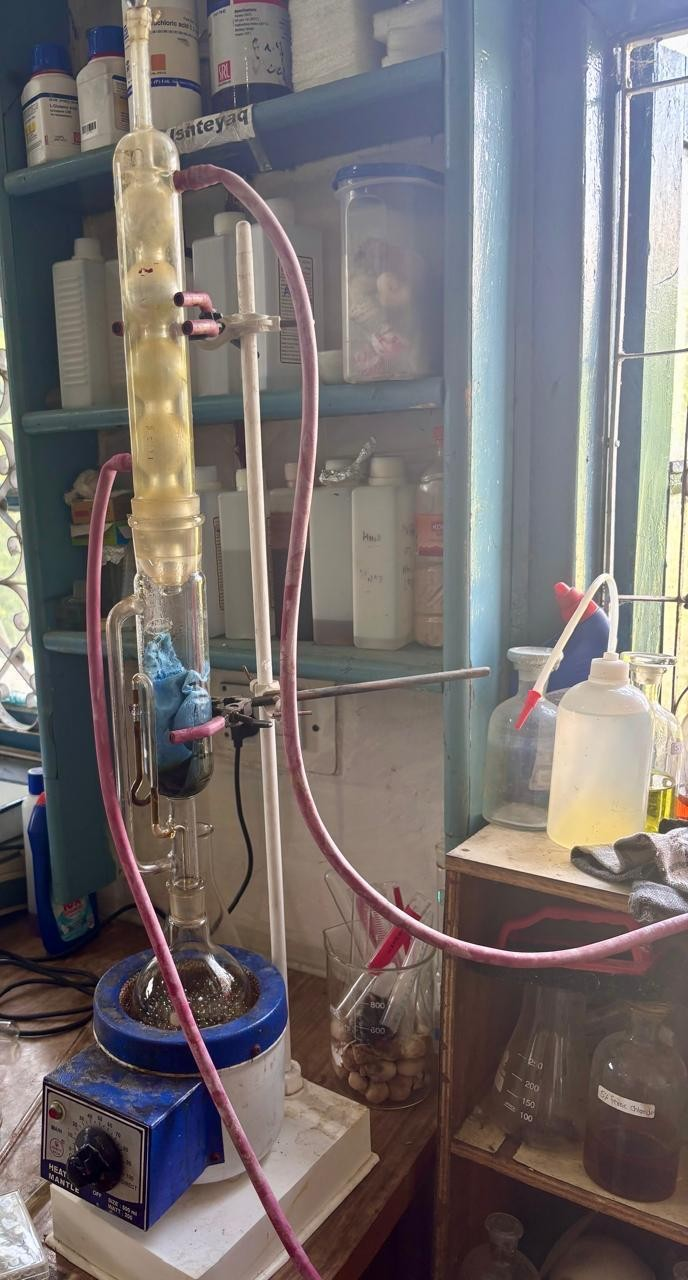
\includegraphics[width=0.55\textwidth]{figures/fig_soxhlet_bench.jpg}
  \caption{Extraction assembly on the laboratory bench: heating mantle, extractor, condenser, and water lines.}
  \label{fig:soxhlet_bench}
\end{figure}

\section{Source of bacterial strains}
\label{sec:bacterial_maintenance}

Clinical pathogenic bacterial strains of \textit{Escherichia coli}, \textit{Pseudomonas aeruginosa}, and \textit{Klebsiella pneumoniae} were obtained from the Advanced Research Laboratory, Department of Zoology, University of Kashmir (\autoref{fig:pure_cultures}, \autoref{fig:ecoli_plate}; additional culture plates in \autoref{app:plate_gallery}). Stocks were maintained on Luria--Bertani (LB) agar. A well-isolated colony of each organism was grown in LB broth at \qty{37}{\celsius} and used to seed a confluent lawn on LB agar plates.

\begin{figure}[htbp]
  \centering
  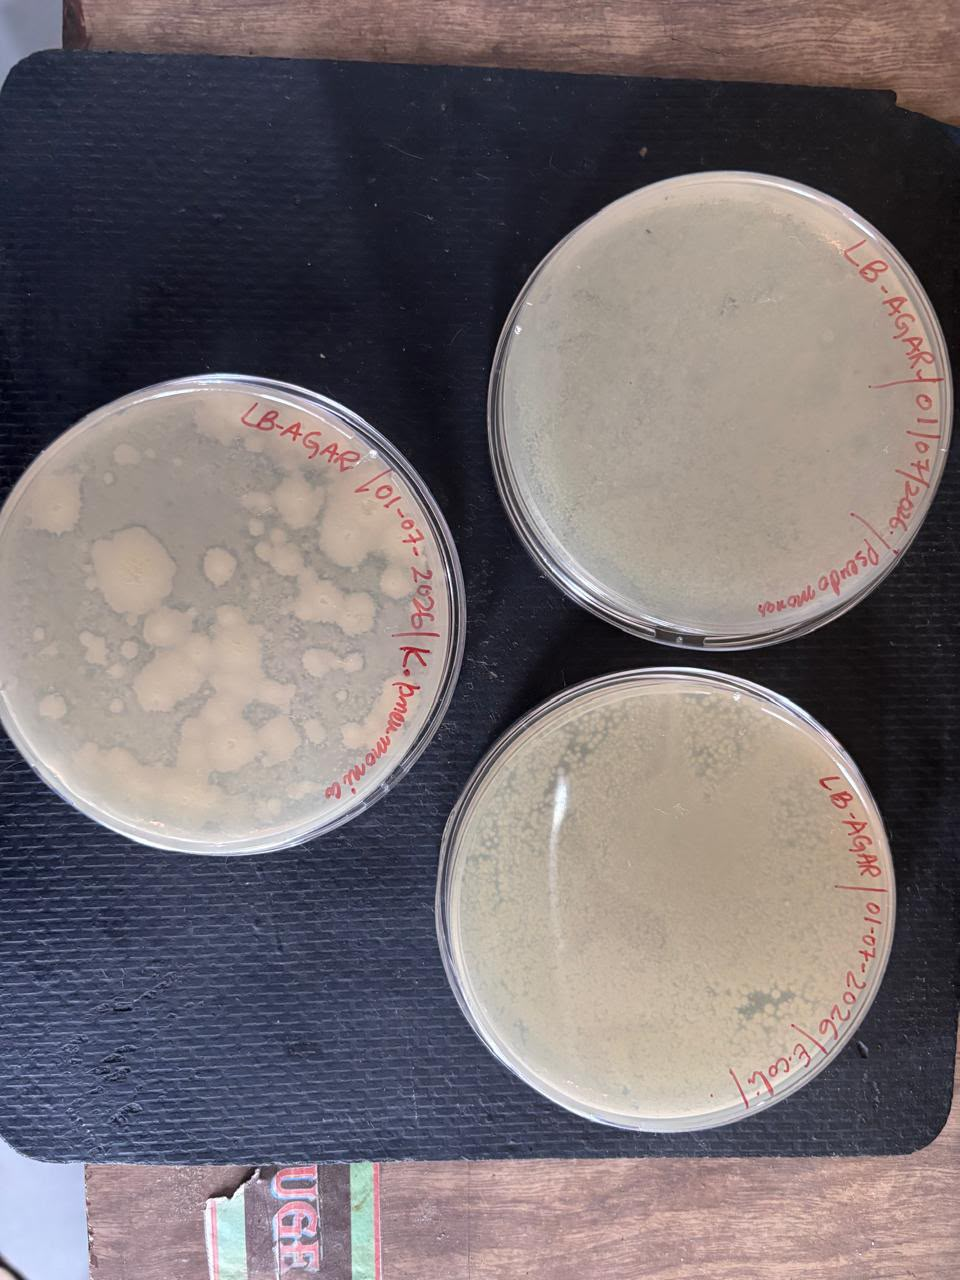
\includegraphics[width=0.82\textwidth]{figures/fig6_pure_cultures.jpg}
  \caption{Pure cultures on LB agar (01-07-2026): \textit{K.\ pneumoniae} (left), \textit{Pseudomonas} (top right), \textit{E.\ coli} (bottom right).}
  \label{fig:pure_cultures}
\end{figure}

\begin{figure}[htbp]
  \centering
  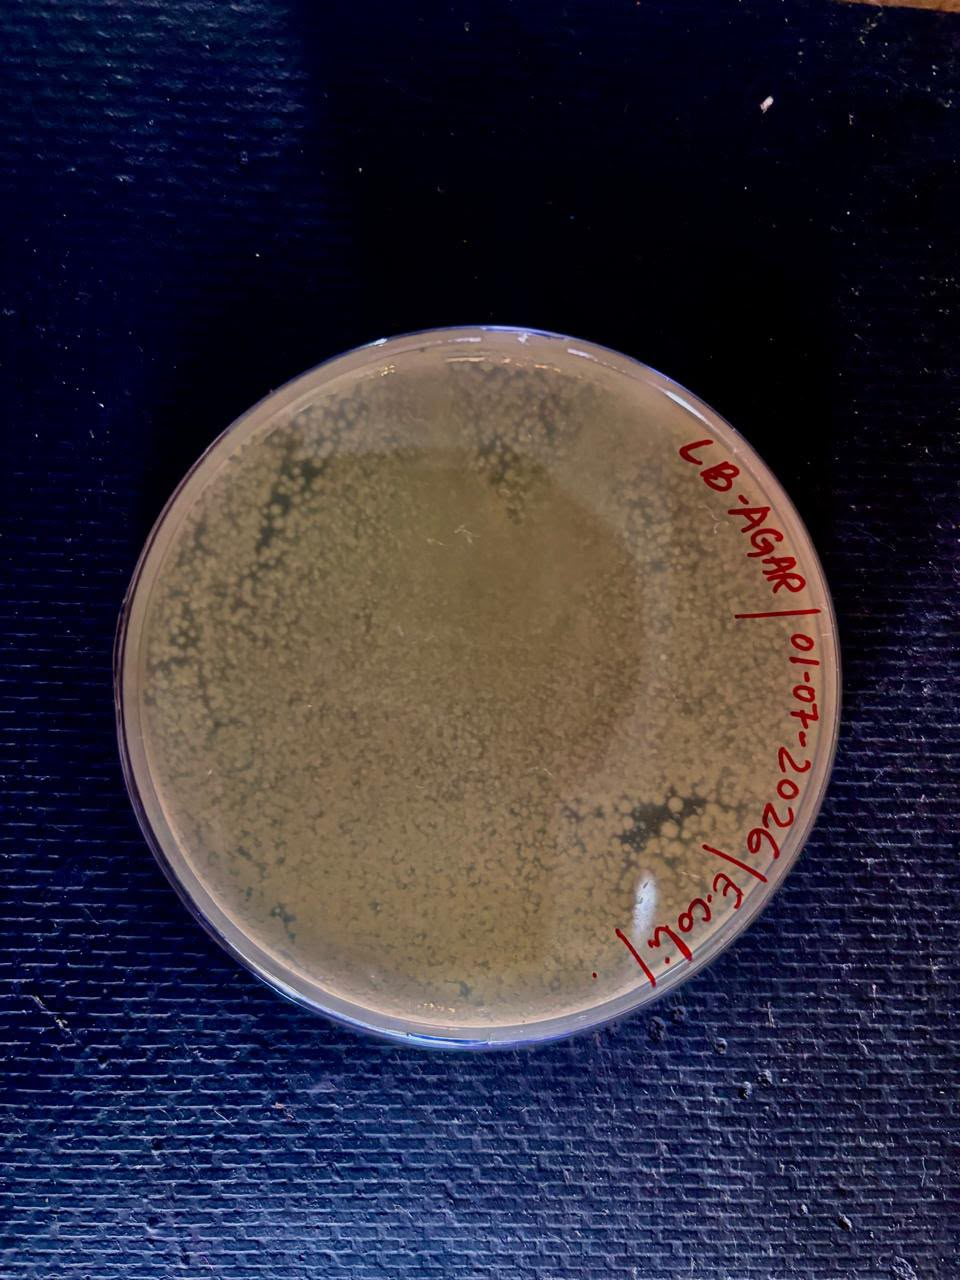
\includegraphics[width=0.72\textwidth]{figures/fig7_ecoli_plate.jpg}
  \caption{Confluent \textit{E.\ coli} culture on LB agar (01-07-2026).}
  \label{fig:ecoli_plate}
\end{figure}

\section{Qualitative phytochemical screening}
\label{sec:phytochem_methods}

The aqueous extract was screened by standard colour tests \citep{harborne1998}. Results are presence or absence only (\autoref{ch:results}; \autoref{fig:phytochem}).

\begin{description}
  \item[Phenolics.] A few drops of 10\% ferric chloride were added to the extract. A bluish-black colour was taken as positive.
  \item[Flavonoids.] A few drops of 10\% sodium hydroxide were added (alkaline reagent test). A yellow colour was taken as positive.
  \item[Alkaloids.] Mayer's reagent was added to the extract. A dull white precipitate was taken as positive.
  \item[Saponins.] Extract was mixed with water and shaken (foam test). Persistent foam was taken as positive.
  \item[Tannins.] A few drops of ferric chloride were added. Dark blue or greenish-black colour was taken as positive.
  \item[Terpenoids.] Extract was treated with thionyl chloride (Salkowski variant). A pink colour was taken as positive.
\end{description}

Carbohydrates (Fehling's), phytosterols (Salkowski with chloroform and sulphuric acid), and quinones (sulphuric acid) were recorded on the same laboratory sheet and are tabulated with the six classes above.

\begin{figure}[htbp]
  \centering
  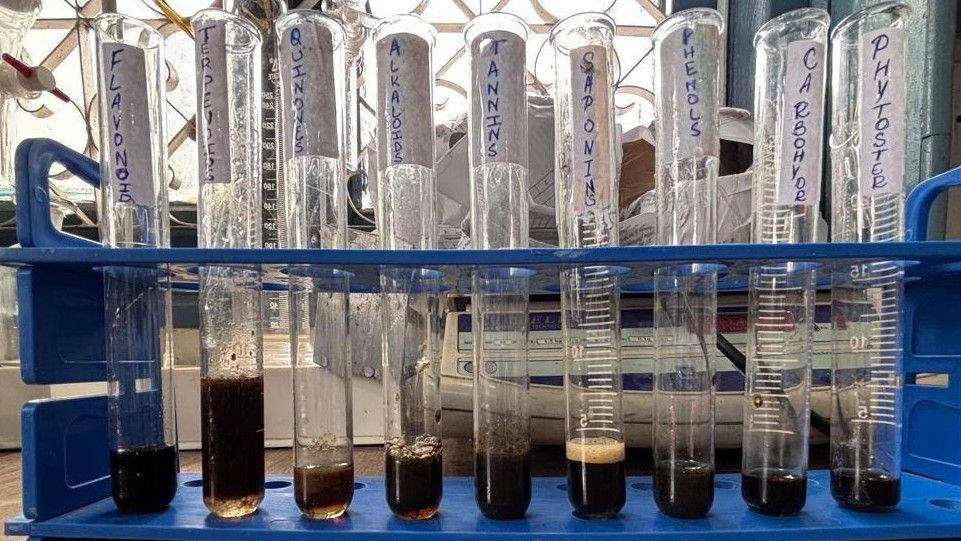
\includegraphics[width=0.78\textwidth]{figures/fig_phytochem.jpg}
  \caption{Qualitative phytochemical tests of the aqueous \textit{D.\ inermis} extract.}
  \label{fig:phytochem}
\end{figure}

\section{Antibacterial assay (disc diffusion)}
\label{sec:susceptibility_testing}

Antibacterial activity was measured by disc diffusion \citep{bauer1966,balouiri2016} on LB agar (\autoref{fig:gen5_disc}, \autoref{fig:c1_c2_unlabelled}). Two extract loads were used:

\begin{itemize}
  \item C1: \qty{50}{\milli\gram\per\milli\litre};
  \item C2: \qty{100}{\milli\gram\per\milli\litre}.
\end{itemize}

The positive control was a commercial gentamicin 5 disc (5\,\textmu g). The negative control was distilled water. Sterile LB agar plates were swabbed with the test culture. Discs loaded with C1, C2, or distilled water, and the gentamicin disc, were placed on the lawn. Plates were incubated at \qty{37}{\celsius} for 24\,h. Each organism $\times$ treatment combination was run in triplicate.

\begin{figure}[hbt!]
  \centering
  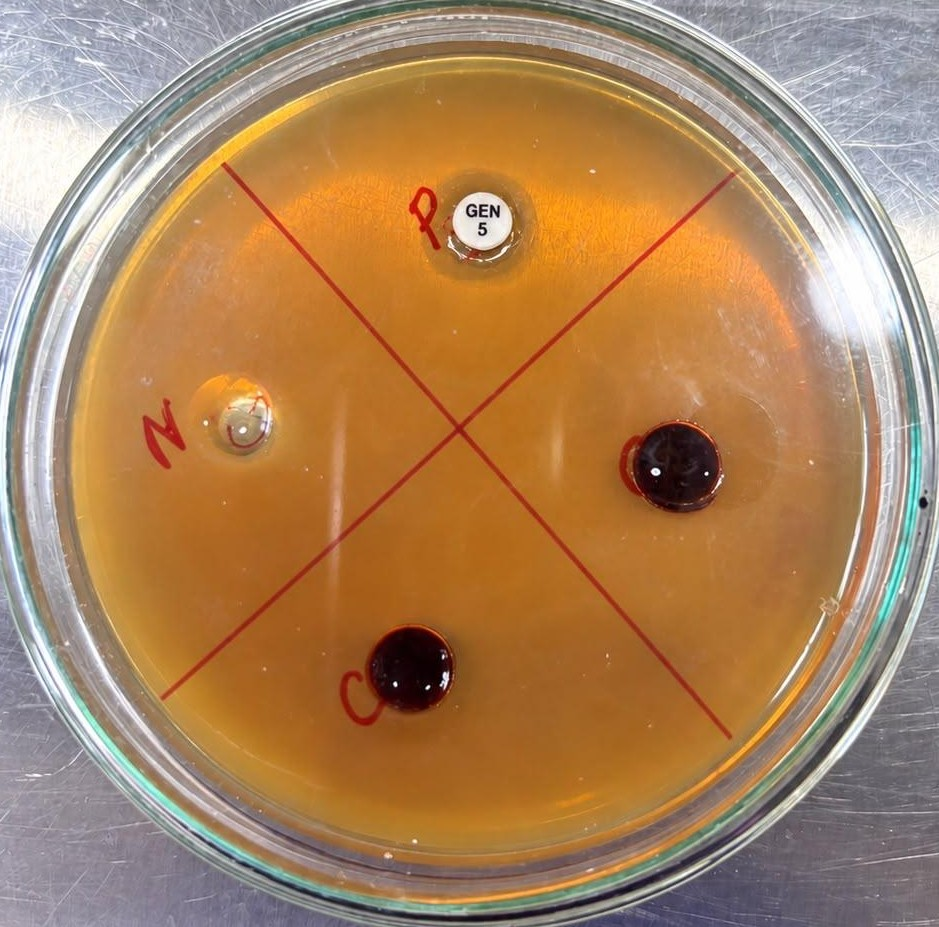
\includegraphics[width=0.62\textwidth]{figures/fig_gen5_disc.jpg}
  \caption{Disc-diffusion plate. The antibiotic disc is labelled GEN~5 (gentamicin 5\,\textmu g). N marks the distilled-water control. The lid does not name the organism.}
  \label{fig:gen5_disc}
\end{figure}

\begin{figure}[hbt!]
  \centering
  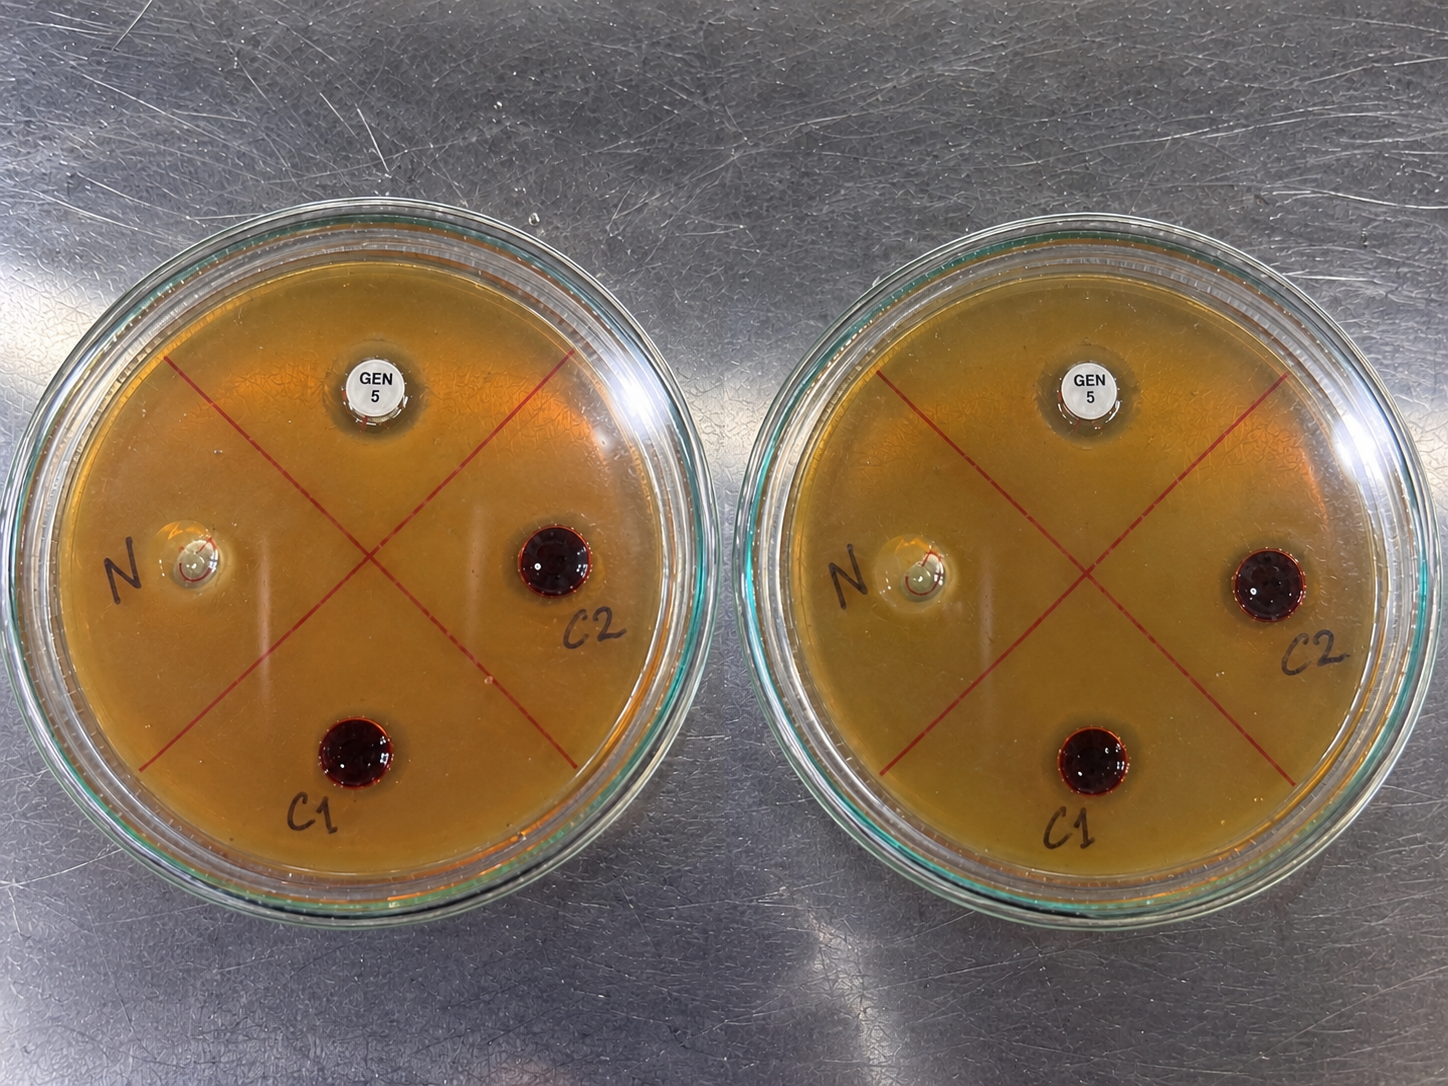
\includegraphics[width=0.78\textwidth]{figures/fig_c1_c2_unlabelled.png}
  \caption{Assay plates showing the C1, C2, N, and GEN~5 layout. The lids do not name the organism.}
  \label{fig:c1_c2_unlabelled}
\end{figure}

\section{Measurement of the zone of inhibition}
\label{sec:zoi_measurement}

After incubation, the diameter of complete clearing around each disc was measured in millimetres with a transparent ruler. \textbf{The zone of inhibition was measured inclusive of the disc.} Values are reported as mean $\pm$ standard deviation of three independent plates. A distilled-water control with no clearing was recorded as zero. Extract zones are described; they are not classified as susceptible or resistant \citep{vanvuuren2019}.
